%\documentclass{article}
%
%\usepackage{tikz}
%\usepackage{tikz-3dplot}
%\usetikzlibrary{calc}
%\usetikzlibrary{patterns}
%\usetikzlibrary{intersections}
%\usetikzlibrary{arrows}
%\tikzset{>=latex}
%
%\begin{document}
%
%\begin{figure}[!h]
%\begin{center}

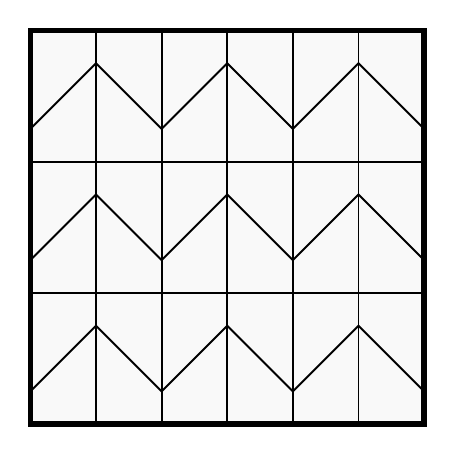
\begin{tikzpicture}[scale = 5.]
	\coordinate[](a) at (0,0);
	\coordinate[](b) at (1,0);	
	\coordinate[](c) at (1,1);
	\coordinate[](d) at (0,1);
	
	\pgfmathsetmacro{\h}{1}	
 	\pgfmathsetmacro{\dh}{1/6}
	
	% Trave
	\filldraw[fill=gray!5!white, line width=2pt, draw=black] 
	(a) -- (b) -- (c) -- (d) -- cycle;

	\begin{scope}[]
	\foreach \x in {1,3,...,5}
	{
	\draw[line width=0.7pt, draw=black] 
	(0, \x*\dh-\dh/2) -- (\dh, \x*\dh+\dh/2) -- (2*\dh, \x*\dh-\dh/2) -- 
	(3*\dh, \x*\dh+\dh/2) -- (4*\dh, \x*\dh-\dh/2) -- (5*\dh, \x*\dh+\dh/2)
	-- (6*\dh, \x*\dh-\dh/2);
	}
	\end{scope}
	
	\begin{scope}[]
	\foreach \x in {1,2,...,5}
	{
	\draw[line width=0.7pt, draw=black] (\x*\dh,  0) -- (\x*\dh,\h);
	}
	\end{scope}
	
	\begin{scope}[]
	\foreach \x in {2,4,...,5}
	{
	\draw[line width=0.7pt, draw=black] (0, \x*\dh) -- (\h, \x*\dh);
	}
	\end{scope}	
	
	
		
\end{tikzpicture}
%\end{center}
%\caption{Square Problem (irregular mesh)}
%\end{figure}
%
%\end{document}